%%%%%%%%%%%%%%%%%%%%%%%%%%%%%%%%%%%%%%%%%%%%%%%%%%%%%%%%%%%%%%%%%%%%
%% I, the copyright holder of this work, release this work into the
%% public domain. This applies worldwide. In some countries this may
%% not be legally possible; if so: I grant anyone the right to use
%% this work for any purpose, without any conditions, unless such
%% conditions are required by law.
%%%%%%%%%%%%%%%%%%%%%%%%%%%%%%%%%%%%%%%%%%%%%%%%%%%%%%%%%%%%%%%%%%%%

\documentclass[
  digital, %% This option enables the default options for the
           %% digital version of a document. Replace with `printed`
           %% to enable the default options for the printed version
           %% of a document.
  notable,   %% Causes the coloring of tables. Replace with `notable`
           %% to restore plain tables.
  lof,     %% Prints the List of Figures. Replace with `nolof` to
           %% hide the List of Figures.
  lot,     %% Prints the List of Tables. Replace with `nolot` to
           %% hide the List of Tables.
  %% More options are listed in the user guide at
  %% <http://mirrors.ctan.org/macros/latex/contrib/fithesis/guide/mu/fi.pdf>.
]{fithesis3}
%% The following section sets up the locales used in the thesis.
\usepackage[resetfonts]{cmap} %% We need to load the T2A font encoding
\usepackage[T1,T2A]{fontenc}  %% to use the Cyrillic fonts with Russian texts.
\usepackage[
  main=english, %% By using `czech` or `slovak` as the main locale
                %% instead of `english`, you can typeset the thesis
                %% in either Czech or Slovak, respectively.
  slovak %% The additional keys allow
]{babel}        %% foreign texts to be typeset as follows:
%%
%%   \begin{otherlanguage}{german}  ... \end{otherlanguage}
%%   \begin{otherlanguage}{russian} ... \end{otherlanguage}
%%   \begin{otherlanguage}{czech}   ... \end{otherlanguage}
%%   \begin{otherlanguage}{slovak}  ... \end{otherlanguage}
%%
%% For non-Latin scripts, it may be necessary to load additional
%% fonts:
\usepackage{paratype}
\def\textrussian#1{{\usefont{T2A}{PTSerif-TLF}{m}{rm}#1}}
%%
%% The following section sets up the metadata of the thesis.
\thesissetup{
    date          = 2017/06/04, %\the\year/\the\month/\the\day,
    university    = mu,
    faculty       = fi,
    type          = bc,
    author        = Lenka Svetlovská,
    gender        = f,
    advisor       = {RNDr. Andriy Stetsko, Ph.D.},
    title         = {Security and cryptography in GO},
    TeXtitle      = {Security and cryptography in GO},
    keywords      = {keyword1, keyword2, ...},
    TeXkeywords   = {keyword1, keyword2, \ldots},
    bib           = example.bib,
}
\thesislong{abstract}{
    This is the abstract of my thesis, which can

    span multiple paragraphs.
}
\thesislong{thanks}{
    This is the acknowledgement for my thesis, which can

    span multiple paragraphs.
}
\usepackage{makeidx}      %% The `makeidx` package contains
\makeindex                %% helper commands for index typesetting.
%% These additional packages are used within the document:
\usepackage{paralist} %% Compact list environments
\usepackage{amsmath}  %% Mathematics
\usepackage{amsthm}
\usepackage{amsfonts}
\usepackage{url}      %% Hyperlinks
\usepackage{markdown} %% Lightweight Markup

%added usepackages
\usepackage{rotating} %rotate table
\usepackage{longtable} %rozdelit tabulku na viac stran

\usepackage[table]{xcolor}
\usepackage{array}
\newcolumntype{P}[1]{>{\centering\arraybackslash\columncolor[HTML]{F2F2F2}}m{#1}} %grey{E9E9E9}
%\newcolumntype{Q}[1]{>{\centering\arraybackslash\columncolor[HTML]{FFF0F0}}m{#1}} %pink
\newcolumntype{Q}[1]{>{\centering\arraybackslash}m{#1}}
%\definecolor{myColor}{RGB}{255,240,240} %pink
\definecolor{myColor2}{rgb}{0.95,0.95,0.92}%{RGB}{233,233,233} %grey
\usepackage[flushleft]{threeparttable} %note in table
\usepackage{enumitem}
\usepackage{graphicx,lipsum,wrapfig} %obrazok obtekany textom
\usepackage{footnote}
\usepackage{listings} %programovacia cast + nasledovne nastavenia
\usepackage{color}
%New colors defined below
\definecolor{codegreen}{rgb}{0,0.6,0}
\definecolor{codegray}{rgb}{0.5,0.5,0.5}
\definecolor{codepurple}{rgb}{0.58,0,0.82}
\definecolor{backcolour}{rgb}{0.95,0.95,0.92}
%Code listing style named "mystyle"
\lstdefinestyle{mystyle}{
  backgroundcolor=\color{backcolour},   commentstyle=\color{codegreen},
  keywordstyle=\color{magenta},
  numberstyle=\tiny\color{codegray},
  stringstyle=\color{codepurple},
  basicstyle=\footnotesize,
  breakatwhitespace=false,         
  breaklines=true,                 
  captionpos=b,                    
  keepspaces=true,                 
  numbers=left,                    
  numbersep=5pt,                  
  showspaces=false,                
  showstringspaces=false,
  showtabs=false,                  
  tabsize=2
}
%"mystyle" code listing set
\lstset{style=mystyle}

\usepackage{verbatim} %comment


\begin{document}
\chapter{Introduction}


\chapter{Basic Terms}
In this chapter, I will define the basic terms which are necessary to an understanding of the 
text presented in the following chapters. First I will describe the structure of certificates, 
standard X.509, certificate authority and signing process. I will explain self-signed certificate and formats. Finally, I will describe protocols SSL/TLS and TLS pre-shared key (TLS\_PSK) 
algorithm used in the application.

\begin{comment}

\section{Cryptography}
Cryptography is the study of mathematical techniques related to aspects of information
security such as confidentiality, data integrity, entity authentication, and data origin
authentication \cite{menezes1996handbook}.Today we talk about computer security which consists 
in the fact that the attacker does not have enough computational strength and time to decode 
the cipher.

\subsection{Symmetric Cryptography}
Symmetric encryption, as the name suggests, means that the encryption and decryption of 
plaintext are based on sharing a together secret - keys.
Symmetric ciphers could be divided into block and stream. Stream ciphers encrypt each 
character of plaintext separately, usually one bit. Block ciphers encrypt plaintext into 
blocks with fixed bit length \textit{n}.

The main disadvantage of symmetric cryptography is the necessity of a large number of keys 
and need of their distribution. For example, for together communication \textit{n} operators 
need to have \[ \frac{n * (n - 1)}{2}\] keys. It means that for the encrypted communications 
of mid-size company with 50 employees, it would need to share 1225 different keys. 

On the other hand, the advantage is the low computational complexity of symmetric ciphers. 
Their using is also useful in cases where the encrypted data are not sent anywhere, for 
example, to protect files on a personal computer.
 
\subsection{Asymmetric Cryptography}
Asymmetric cryptography allows data encryption and particularly the implementation of the 
digital signature. Each entity has two keys. The first is the private key that is used to 
decrypt a message or create a digital signature. It must be kept secret. The second key is 
public which is used for encryption and authentication of the digital signature. Of course, 
there is impossible to derive the private key from the public key \cite{dostalek2016velky}.

The main advantages of asymmetric cryptography are mainly a smaller number of keys than 
symmetric cryptography. If each entity has one public and one private key, it means that for 
\textit{n} entities are needed \textit{2n} keys. In the same situation as in the previous 
example, a company of 50 employees would need to ensure the safety of 100 keys, which is 
substantially less than 1225.

The biggest disadvantage of asymmetric cryptography is its slowness compared with symmetric 
cryptography. Therefore, they are most often used together, while the text is encrypted with a 
random symmetric encryption key. The key is encrypted using asymmetric ciphers. In the case of 
a digital signature, the first is created the fixed length hash of the message and then it is 
signed using asymmetric cryptography.

\subsection{Hash Function}
Hash functions are one of the basic elements of modern cryptography, often called one-way 
hash function.

Hash functions are effectively designed display binary strings unlimited length to binary 
strings a fixed length, called hash value. For a perfect hash function that has \textit{n}-bit 
hash value, there is a chance that a randomly selected string will be displayed on specific 
hash value $2^{-n}$. The basic idea of hash functions is that the hash value should serve as a 
representative of the input string. Hash function suitable for use in cryptography is usually 
chosen so that it is computationally very difficult find two different input strings that have 
the same hash value. If it succeeds in these two find strings, we say that we found a 
collision. 
Likewise, it should be computationally very difficult to find for a hash value corresponding 
to the input string. Using hash functions are used frequently to check the integrity of data 
and for digital signing of data \cite{piper2006kryptografie}.

ITEMIZE

\end{comment}

\section{Certificate}
Certificate is digitally signed data structure whose basis includes a public key of
certificate owner. There are some standards of the certificate structure (X.509, EDI, WAP, 
etc.). The Internet is based on standard X.509 version 3, which was issued by the ITU \cite{dostalek2016velky}. %For the needs of the Internet, there is created an Internet profile of X.509 in the relevant RFC. Current Internet profile certificate is standard RFC-5280 \cite{dostalek2016velky}.

\subsection{Standard X.509}
Standard X.509 was originally designed as an authentication framework for X.500 
directories. They have a hierarchical structure and the individual attributes can be assigned to 
individual computers of companies or individual printers \cite{schmeh2006cryptography}. % That is, each entity can be clearly identified, and each can have its private and public key.
Certificate X.509, see Figure \ref{fig:certificate}.

\begin{comment}
\vskip 0.1in
The first version of the X.509 standard was already appeared in 1988 as the first proposal for 
PKI \cite{schmeh2006cryptography}. The first version was very simple and today is already 
inadequate. It contained only 7 fields:
\vskip 0.1in
\begin{itemize}[leftmargin=2em,rightmargin=1em,itemsep=0.75\parskip,parsep=0em,topsep=0em,partopsep=0em]
\item certificate version;
\item certificate series number;
\item algorithm which signed certificate;
\item name of certification authority which certificate released;
\item identity of certificate owner;
\item public key of certificate owner;
\item certificate validity.
\end{itemize}
\vskip 0.1in
The second version was introduced five years later in 1993 and brought only minimal changes. 
Fields which was needed in this version, still missing \cite{schmeh2006cryptography}. It 
contained only two new fields:
\vskip 0.1in
\begin{itemize}[leftmargin=2em,rightmargin=1em,itemsep=0.75\parskip,parsep=0em,topsep=0em,partopsep=0em]
\item unique identifier of the certificate owner;
\item unique identifier of the certification authority.
\end{itemize}
\vskip 0.1in
The third version was introduced in 1996. Its biggest and most important benefit is to support 
the expansion. It eliminates the major shortcomings of the two previous versions \cite{housley2002internet}.
\end{comment}
\begin{figure}[th]
	\centering
	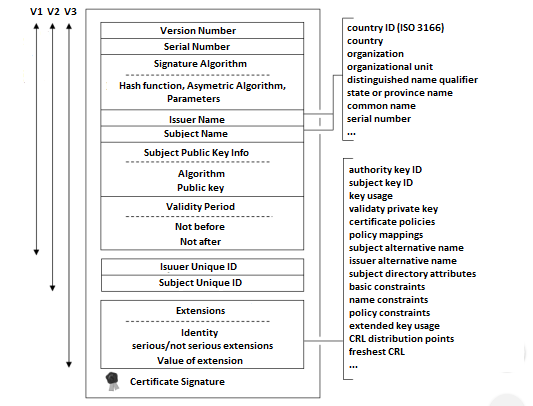
\includegraphics[width=1.05\textwidth]{certificate}
	\caption{Structure X.509 Certificate}
	\label{fig:certificate}
\end{figure}

\subsection{Certificate Authority}
The Certificate Authority (CA) is an independent third party which issues certificates.

In other words, the CA is an institution that inspects the certificate request and issues whose 
validity is verifiable using the responsive public key. The CA was created %(in 1998 in order) 
to ensure secure encryption through a certified public key and guarantee the validity of the 
digital signature. The CA also ensures their validity revocation. The CA is truly credible, must 
be impartial and, if it is possible, should be subordinate to any higher CA. Subordination means 
that it identifies the usage of certificates signed by the higher certificate authority 
\cite{dostalek2016velky}.

Root CAs, certificate authorities at the highest level, use the certificate signed by 
themselves (self-signed certificate).

\nocite{singh2003kniha}

\subsection{Self-signed Certificate}
The self-signed certificate is a certificate which the applicant issues by himself. The 
self-signed certificate has the same data structure as a certificate issued by CA. This 
certificate is recognized according to identical item Subject and item Issuer.

As proof of the private key possession by the user, the self-signed certificate uses a 
digital signature which was made by the private key belonging to the public key 
in the certificate. Verification of the signature is carried out through a public key in the 
actual certificate \cite{dostalek2016velky}.

\begin{comment}
Self-signed certificate is used by software internally. While the applicant generates CSR to 
be issued by the CA, the public key must be kept by the applicants. In this case, the public 
key is often maintained like a self-signed certificate. Subsequently it is rewritten by the 
certificate.
\end{comment}

\subsection{Certificate Signing Request}
The certificate applicant can apply CA to sign certificate by submitting a data structure called a 
certificate request (CSR) \cite{dostalek2016velky}. The most common format is PKCS\#10. The CSR 
should include:
\begin{itemize}[leftmargin=2em,rightmargin=1em,itemsep=0.75\parskip,parsep=0em,topsep=0em,partopsep=0em]
\item Applicant ID
\item The public key
\item Evidence of the possession of the private key
\item Other information that the user wishes to insert certificate
\item May contain evidence of the generation of paired data
\item Data necessary for billing (in case issuance of certificates is paid)
\item Passwords for communication with CA:
  \begin{itemize}[leftmargin=2em,rightmargin=1em,itemsep=0.75\parskip,parsep=0em,topsep=0em,partopsep=0em]
  \item One-time password for issuing the certificate
  \item One-time password for certificate revocation
  \item Permanent password for personal (non-electronic) communication between user and CA
  \item Phrase (in case losing all passwords) 
  \end{itemize}
\end{itemize} 

The certificate authority must fill individual fields of the certificate before it signs the 
result digitally. The CA takes CSR, checks completed fields and fills two important fields called validity period - the time while the certificate is valid - which are shown as: not before, not after. The CA can also add extensions, such as Subject Alternative Name, information 
about CA, etc. (see figure \ref{fig:certificate}).

\subsection{Formats PEM and DER}
The PEM (Privacy Enhanced Mail) is a Base64 encoded DER certificate. It is designed 
to be safe for inclusion in ASCII or even rich-text documents. This means that we can simply copy 
and paste the content of a pem file to another document and back. Following figure is a sample 
PEM file containing a private key and a certificate \ref{fig:vzorPEM-DER}.

\begin{figure}[th]
	\centering
	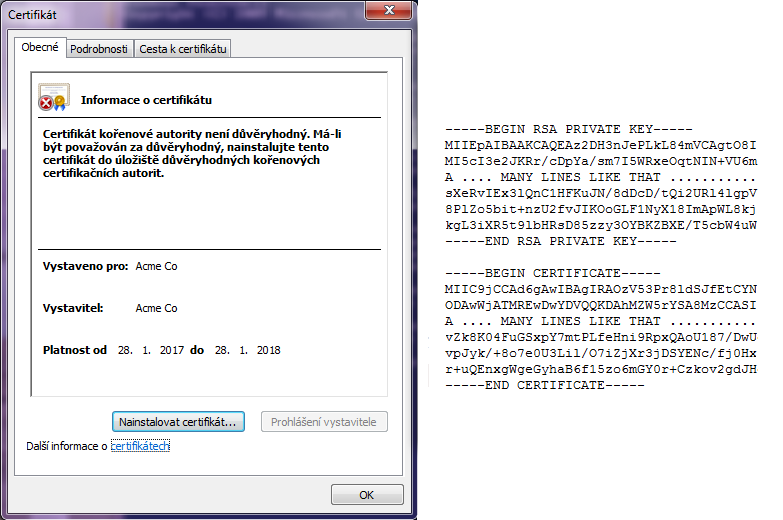
\includegraphics[width=1\textwidth]{pem-der}
	\caption{A sample example of certificate view}
	\label{fig:vzorPEM-DER}
\end{figure}

A certificate or key must start with header where the number of dashes is meaningful, and must 
be correct. A single PEM file can contain a number of certificates and a key, for example, a 
single file with public certificate, intermediate certificate, root certificate or private key 
\cite{howToSsl}.

The DER (Distinguished Encoding Rules) is a binary form of ASCII PEM format 
certificate. All types of certificates and private keys can be encoded in DER format, its 
information is stored in the binary DER for ASN.1 and applications providing RSA, SSL and TLS 
should handle DER encoding to read in the information. DER can not contain more then one certificate \cite{bakker_2014}.

\section{Protocol SSL/TLS}
Protocol SSL/TLS is used for communication security between the client and the server. It 
creates a framework for the use of encryption and hash functions.

Protocol SSL was developed by Netscape Communications which published three versions. The first 
version was only a test, the second has been used in practice. However, it still contained 
security vulnerabilities, the most important was susceptibility to attack \textit{man in the 
middle} \cite{oppliger2003security}. %zdroj?? https://scholar.google.sk/scholar?q=Security+Technologies+for+the+World+Wide+Web&btnG=&hl=sk&as_sdt=0%2C5 
The third version was introduced in 1996 and its specification could be found in the document 
\textit{The SSL Protocol Version 3.0} \cite{freier2011secure}. From this version was created TLS 
protocol which is currently the most widespread and supported \cite{oppliger2003security}. 
There are currently three versions which have only minimal differences. TLS version 1.3 is a draft 
already used in multiple locations \cite{draft-tls}. For example, the forthcoming \textit{OpenSSL 1.1.1} release will include support for \textit{TLSv1.3} \cite{foundation2}.

Protocol SSL/TLS provides authentication of the two communicating parties by using asymmetric 
encryption, message integrity by using MAC and confidentiality by encrypting all 
communications by selected symmetric cipher.

Protocol SSL/TLS is located between the application and the transport layer reference ISO/OSI 
model and consists of two main parts. They are \textit{The Record Layer Protocol} and 
\textit{Handshake Protocol} \cite{oppliger2003security}. %Part of HP are two auxiliary protocols - \textit{Change Cipher Specification Protocol} (CCSP) and \textit{Alert Protocol} (AP) \cite{oppliger2003security}.

\subsubsection{Record Layer Protocol (RLP)}

RLP processes application data, performs fragmentation, compression and data encryption. On the 
other hand, it decrypts the data again and verifies the checksums. RLP does not care about the 
type of encryption algorithm or encryption key setting. This information is from HP.

\subsubsection{Handshake Protocol (HP)}
HP is activated immediately after establishment the connection and provides identification of 
communicating parties, negotiation of cryptographic algorithms, compression algorithms and other 
attributes. Then it creates \textit{a master secret} from which are derived encryption keys, 
initiation vectors and the MAC. The process of the protocol is:

\begin{enumerate}
\item The client sends a \textit{ClientHello} message to the server, along with the client's random value and supported cipher suites.
\item The server responds by sending a \textit{ServerHello} message to the client, along with the server's random value.
\item The server sends its certificate to the client for authentication and may request a certificate from the client. The server sends the \textit{ServerHelloDone} message.
\item If the server has requested a certificate from the client, the client sends it.
\item The client creates a random \textit{Pre-Master Secret} and encrypts it with the public key from the server's certificate, sending the encrypted \textit{Pre-Master Secret} to the server.
\item The server receives the \textit{Pre-Master Secret}. The server and client each generate the \textit{Master Secret} and session keys based on the \textit{Pre-Master Secret}.
\item The client and the server exchange the \textit{Finished} messages.
%\item %The client sends \textit{ChangeCipherSpec} notification to server to indicate that the client will start using the new session keys for hashing and encrypting messages. 
%Client sends \textit{ClientFinished} message.
%\item %Server receives \textit{ChangeCipherSpec} and switches its record layer security state to symmetric encryption using the session keys. 
%Server sends \textit{ServerFinished} message to the client.
\end{enumerate}

Client and server can now exchange application data over the secured channel they have established. All messages sent from client to server and from server to client are encrypted using session key \cite{handshakeprotocol}.

\begin{comment}
\begin{enumerate}
\item The client wants to connect to the server and sends \textit{ClientHello}, which contains 
the highest number of version supported by SSL/TLS, the number of session (it is empty if it 
is a new session), the list of supported ciphers and compression methods and a random number.
\item The client waits for a response in the form of a report \textit{ServerHello}, which will 
contain the highest number of versions of SSL/TLS, which is supported by server and client. It 
will also contain encryption and compression method, which are selected from the list received 
in step one, a random number and its public key certificate (the server can also request 
client authentication).
\item The client validates the server certificate and sends a request to exchange keys. At the end the server and client share a common \textit{premaster secret}. \textit{The master secret} is derived from it. The \textit{ClientHello} and \textit{ServerHello} are derived from the master secret.
\item From this moment, the communication has been encrypted and the client sends a message that ends with this phase. In case the server required the client authentication, it has been carried out in this step. Finally, the server sends a confirmation used ciphers and message about the completion of this phase, thereby HP ends.
\end{enumerate}
\end{comment}

%\textit{Change Cipher Specification Protocol} is a simple protocol that contains only a single message. It says there was the change of the encryption parameters and now only new ones will be used. It could be also called after the end of the initial phase.

%\textit{Alert protocol} provides the transmission of warning in case of any problem in communication - it contains an array of warning severity and description of the problem.

\begin{comment}
TLS uses public key certificates for authentication. To establish a TLS connection are used 
symmetric keys (later called pre-shared keys or PSKs), shared in advance among the 
communicating parties \cite{eronen2005pre}.
\end{comment}

\subsection{PSK Key Exchange Algorithm}\label{pskAlgorithm}
The cipher suites with the PSK key exchange algorithm use only symmetric key algorithms and 
are particularly suitable for performance-constrained environments where both ends of the 
connection can be controlled. The cipher suites are intended for a rather limited set of 
applications, usually involving only a very small number of clients and servers.

\begin{enumerate}
\item The client indicates to use pre-shared key authentication by including one or more PSK cipher suites in the \textit{ClientHello} message. 
\item If the TLS server also wants to use pre-shared keys, it selects one of the PSK cipher suites and places it in \textit{the ServerHello} message. The server can provide a "PSK identity hint" in the \textit{ServerKeyExchange} message. If no hint is provided, the \textit{ServerKeyExchange} message is omitted.
\item The client indicates which key to use by including a "PSK identity" in the \textit{ClientKeyExchange} message.
\item The \textit{Certificate} and \textit{CertificateRequest} payloads are omitted from the response.
\item The TLS handshake is authenticated using the \textit{Finished} messages. 
\end{enumerate}

\begin{figure}[th]
	\centering
  	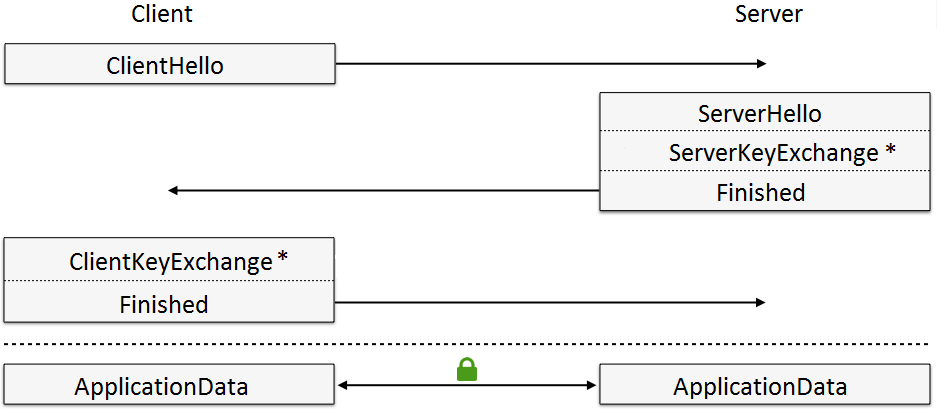
\includegraphics[width=1.05\textwidth]{psk-edited}%{tls13-hs-resumption}%{psk}
   \caption{TLS\_PSK Key Exchange}
\end{figure}

If the server does not recognize the PSK identity, it may respond with an 
\textit{unknown\_psk\_identity} alert message.  Alternatively, if the server wishes to hide 
the fact that the PSK identity was not known, it may continue the protocol as if the PSK 
identity existed but the key was incorrect: that is, respond with \textit{a decrypt\_error 
alert} \cite{eronen2005pre}. 

\chapter{Language Go}\label{go}
In this chapter I will explain the main characters of language Go and show how to write the 
code. Next I will describe Go libraries called packages and the tool Cgo.

\section{Introduction}
Go is a programming language developed at \textit{Google} in year 2007 and announced in 
November 2009. Many companies have started using Go because of its performance, simplicity, 
ease of use and powerful tooling. Go programming language is a statically-typed language with 
advanced features and a clean syntax \cite{doxsey2016introducing}. It combines the performance 
and security benefits associated with using a compiled language like \textit{C++} with the 
speed of a dynamic language like \textit{Python}. It provides:
\vskip0.1in
\begin{itemize}[leftmargin=2em,rightmargin=1em,itemsep=0.75\parskip,parsep=0em,topsep=0em,partopsep=0em]
\item garbage collector - memory is cleaned up automatically when nothing refers to it 
anymore,
\item fast compilation time - through effective work with addictions individual parts of the 
program and simple grammar,
\item light-weight processes (via go-routines), channels,
\item a rich standard library,
\item easy testing - incorporated directly into the core language,
\item one of the best documentation - a clear and full of examples.
\end{itemize}
\vskip0.1in

Go excluded some features intentionally to keep language simple and concise. There is no 
support for type inheritance, method or operator overloading, circular dependencies among 
packages, pointer arithmetic, assertions nor for generic programming.
\nocite{wiki-go}
\nocite{doxsey2016introducing}

\section{How to Start}\label{howToStart}
\subsection{Installation}
Golang, the go official website, provides the installer of Go to download free for Windows, 
Linux, Mac OS X and FreeBSD. To confirm everything is working, open a terminal and 
type the following:
\begin{lstlisting}
go version
\end{lstlisting}
Upgrading from an older version of Go must be precessed by removing the existing version. 

\subsection{Enviroment}
After installation, it is necessary to set Go to the \textit{\$PATH} environment variable and set the \textit{\$GOROOT} environment variable to point to the directory in which it was installed. The Go toolset uses an environment variable called \textit{\$GOPATH} to find Go source code. 

For example, if you installed Go to your home directory you should add commands like the following to \textit{\$HOME/.profile}:
%Set up your workplace, for example \textit{GOPATH=C:/Projects/Go}.
\begin{lstlisting}
export GOROOT=$HOME/go1.X
export PATH=$PATH:$GOROOT/bin
export GOPATH=$HOME/Projects/go
\end{lstlisting}
\textit{\$GOPATH} has to contain directories \textit{src} and \textit{pkg}.

\begin{comment}
\subsection{First Program}
Traditionally, the first program in any programming language is called a
hello program — a program that simply outputs "Hello World!" to terminal.

Open text editor, create file $hello.go$, and enter the following:
\begin{lstlisting}
package main
import "fmt"
// this is a comment
func main() {
	fmt.Println("Hello World!")
}
\end{lstlisting}
Make sure the file is identical to what is shown here and save it.
\end{comment}

\subsection{Compilation and Arguments}
Go is a compiled language, and like many languages, it makes heavy use of the command
line. Open up a new terminal, set up directory where you saved your file and type in the following for run the file:
\begin{lstlisting}
go run <file-name>.go
\end{lstlisting}
or type in the following to parameterize execution of programs. First must be used go build command to create a binary program.
\begin{lstlisting}
go build <file-name>.go
./<file-name> <arguments>
\end{lstlisting}
In code, $os.Args$ provides access to raw command-line arguments. The first value is the path to the program, and \textit{os.Args[1:]} holds the arguments to the program.
\begin{lstlisting}
argsWithProg := os.Args
argsWithoutProg := os.Args[1:]
arg := os.Args[3]
\end{lstlisting}
Do not forget to import package $os$.
%You should see Hello World! displayed in your terminal.

\begin{comment}
\subsection{Arguments}
Command-line arguments are a common way to parameterize execution of programs. First must be used go build command to create a binary program.
\begin{lstlisting}
go build cmd-arguments.go
./cmd-arguments a b c
\end{lstlisting}
In code, $os.Args$ provides access to raw command-line arguments. The first value is the path to the program, and \textit{os.Args[1:]} holds the arguments to the program.
\begin{lstlisting}
argsWithProg := os.Args
argsWithoutProg := os.Args[1:]
arg := os.Args[3]
\end{lstlisting}
Do not forget to import package $os$.
\end{comment}

\section{Packages}
In Go, source files are organized into system directories called packages. To  develop 
software applications, writing maintainable and reusable pieces of code is very important. Go 
provides the modularity and code reusability through its package system. Go encourages 
programmers to write small pieces of software components through packages, and compose their  
applications with these small packages.

The packages from the standard library are available at the $pkg$ subdirectory of the $\$GOROOT$ 
directory. When we install Go, an environment variable $\$GOROOT$ will be automatically added to 
our system for specifying the Go installer directory. The Go developer community is very 
enthusiastic for developing third-party Go packages. When you develop Go applications, you can 
affect these third-party Go packages \cite{stack_2014}.

When programmers develop executable programs, they will use the package $main$ for making the 
package as an executable program. The package $main$ tells the Go compiler that the package 
should compile as an executable program instead of a shared library. When programmers build 
shared libraries, they will not have any main package and main function in the package.

To download third-party Go packages the following command is used: 
\begin{lstlisting}
go get example/exampleLib
\end{lstlisting}
After installing the exampleLib, put the import statement in programs for reusing the code, as 
shown below:
\begin{lstlisting}
package db
import (
	"example/exampleLib"
	"example/exampleLib/sub"
)
func init {
	// initialization code here    
}
\end{lstlisting}
Third-party Go packages are installed by using this command: 
\begin{lstlisting}
go install
\end{lstlisting}
The go install command will build the package “sub” which will be available at the $pkg$ 
subdirectory of $\$GOPATH$.
\begin{lstlisting}
package main
import (
	"fmt"
	"example/exampleLib/sub"
)
func main() {
    sub.Add("dr","Dart")
    fmt.Println(sub.Get("dr"))
    // code here    
}
\end{lstlisting}

\section{C? Go? Cgo!}\label{cgo}
Cgo allows Go to interoperate with C code. Go source file imports~"C" and it is immediately 
preceded by comment lines which may contain any C code, including function and variable 
declarations and definitions. It is necessary to say that there must be no blank lines in 
between the cgo comment and the import statement. 

\begin{lstlisting}
package main
/*
#include <stdio.h>

void hello() {
	printf("Hello World!\n");
}
*/
import "C"

func main() {
	C.hello()
}
\end{lstlisting}

Cgo allows including own C libraries. The header file $foo.h$, the library implementation 
$foo.c$ and go wrapper $foo.go$ are located in the same package $\$GOPATH/src/foo$. 
\begin{lstlisting}
#cgo CFLAGS: -I/{$GOPATH}/src/foo
#cgo LDFLAGS: -L/{$GOPATH}/src/foo -lfoo
\end{lstlisting}
Go wrapper contains the explicit paths in the cgo flags because of an environment issue where 
libfoo wasn’t found by the Go linker.
\begin{lstlisting} 
go install foo 
\end{lstlisting}
By installing the package everything is prepared for using in Go. Package is called in Go code 
through $import "foo"$.

In order to use Cgo on Windows, it is firstly needed to install a gcc compiler and have 
$gcc.exe$ in $\$PATH$ environment variable before compiling with Cgo will work.

\nocite{cgo-command}
\nocite{bloggolangorg}
\nocite{cgo-wiki}

\nocite{chisnall2012go}
\nocite{balbaert_2012}
\nocite{summerfield_2012}
\nocite{harris_2015}
\nocite{kozyra_2014}

\chapter{Go Packages Analysis} %The analysis of go packages
This chapter contains the overview, evaluate and compare existing cryptographic libraries based on 
their measures and expansion measures important for implementation.

\section{Cryptographic functions}
It was necessary to examine features of language Go related to the security and cryptography, analyze 
libraries which Go contains and also search for available third-party libraries. 

Table \ref{table:analysis} shows analyzed Go package Crypto created by \textit{Golang} and other Go 
packages created by third-parties. Individually items mean:
\vskip0.1in
\begin{itemize}[leftmargin=2em,rightmargin=1em,itemsep=0.75\parskip,parsep=0em,topsep=0em,partopsep=0em]
\item Name - founder nickname (almost all packages are searched on \textit{https://github.com/} where is not published real name of founder or contributors) and name of package.
\item Cryptographic functions - support cryptographic functions, such as symmetric encryption, asymmetric encryption and hash functions (all/sym/asym/hash/unknown).
\item Start of project - a year of creating project with package.
\item Is still opened - the important measure is if contributors still work on the project (Yes/No).
\item Issue tracker system - support of solving bugs, feature requests, tracking todos, and more (Yes/No).
\item Documentation accessibility - assessed on a scale of 0-5 points (5 is the highest) according to own experience to work with the package.
\item Downloads - number of downloads. In case the package is saved on \textit{https://github.com/}, the information about downloads presents value of Fork. Downloads of package Crypto created by Golang is unknown, this package is automatically installed with installing program Go.  
\item License - availability of licenses for free (Yes/Payment). The payment indicates the amount of payment per some period. This case did not occur.
\end{itemize}
\vskip0.1in

\begin{center}
\begin{longtable}[th]{|P{1.6cm}|Q{1cm}P{1cm}Q{1cm}P{1.3cm}Q{1.3cm}P{1.2cm}Q{1.1cm}|}
\caption{Table of cryptographic libraries in Go} \label{table:analysis} \\

\hline \hline
%\rowcolor[HTML]{EFEDED}
Name & Crypto. functions & Start of project & Is still opened & Issue tracker system & Doc. accessibility & Down-loads & License\\ [6ex]
\hline \hline \hline \hline
\endfirsthead

\multicolumn{8}{c}
{{\tablename\ \thetable{} -- continued from previous page}} \\
\hline \hline
%\rowcolor[HTML]{EFEDED}
Name & Crypto. functions & Start of project & Is still opened & Issue tracker system & Doc. accessibility & Down-loads & License \\ [6ex]
\hline \hline \hline \hline
\endhead

\hline \hline
\rowcolor[HTML]{E9E9E9} 
\multicolumn{8}{|r|}{{Continued on next page}} \\ \hline
\endfoot

\hline 
\endlastfoot

golang/ crypto & all & 2009 & Y & Y & 5 & - & Y\\ [3ex]
%go-lang. cat-v.org/ pure-go-libs & N & \footnote{Page ceased updating in October, 2012} & & & & & Y \\ 
%golang libs.com category cryptography & Y & not all & 2012-2016 & some & & & \\
%golang libs.com category security & Y & not all & 2013-2016 & some & & & \\
ory-am/ fosite & asym, hash & 2015 & Y & Y & 4 & 39 & Y \\ [4ex]
square/ go-jose & asym, sym & 2014 & Y & Y & 4 & 70 & Y \\ [4ex]
Shopify/ ejson & hash & 2014 & Y & Y & 3 & 22 & Y \\ [3ex]
mitchellh/ go-mruby & asym & 2014 & Y & Y & 4 & 19 & Y \\ [4ex]
Sermo Digital/ jose & all & 2015 & Y & Y & 4 & 28 & Y \\ [4ex]
mozilla/ tls-observatory & hash & 2014 & Y & Y & 4 & 31 & Y \\ [4ex]
square/ certigo & hash & 2016 & Y & Y & 3 & 12 & Y \\ [3ex]
docker/ libtrust & all & 2014 & N & Y & 4 & 26 & Y \\ [3ex]
dedis/ crypto & sym, hash & 2010 & Y & Y & 4 & 17 & Y \\ [3ex]
dchest/ blake2b & hash & 2012 & N & Y & 4 & 6 & Y \\ [3ex]
enceve/ crypto & hash & 2016 & N & Y & 4 & 1 & Y \\ [3ex]
go-libp2p-crypto & all & 2015 & Y & Y & 4 & 5 & Y \\ [3ex]
dchest/ blake2s & hash & 2012 & N & N & 3 & 3 & Y \\ [3ex]
benburkert/ openpgp & sym, hash & 2012 & N & N & 3 & 0 & Y \\ [4ex]
minio/ sha256-simd & hash & 2016 & Y & Y & 3 & 14 & Y \\ [4ex]
avelino/ awesome-go & un-known & 2014 & Y & Y & 2 & 2287 & Y \\ [4ex]
ethereum/ go-ethereum & all & 2013 & Y & Y & 4 & 1028 & Y \\ [4ex]
chain/ chain & hash & 2015 & Y & Y & 4 & 113 & Y \\ [3ex]
lightning network/lnd & sym, hash & 2015 & Y & Y & 4 & 50 & Y \\ [4ex]
square/ go-jose & asym, hash & 2014 & Y & Y & 4 & 70 & Y \\ [3ex]
dgrijalva/ jwt-go & asym, hash & 2012 & Y & Y & 4 & 226 & Y \\ [3ex]
golang/ oauth2 & asym, hash & 2014 & Y & Y & 4 & 279 & Y \\ [3ex] 
\end{longtable}
\end{center}
%%  Zdroje k tabulke:
%%% https://golanglibs.com/top?q=security
%%% https://golanglibs.com/category/cryptography?sort=top
%%% http://go-lang.cat-v.org/pure-go-libs
%%% https://godoc.org/golang.org/x/crypto
%%% https://golang.org/pkg/
%%% ?

The table \ref{table:analysis} was created based on information available on 
following websites \cite{security-golibrariesAndApps} \cite{cryptography-golibrariesAndApps} 
\cite{crypto-godoc} \cite{packages-thegoprogramminglanguage}. The 
table does not contain packages which do not support any cryptographic functions. Also, 
the table does not contain information from untrusted sources. During the analysis, I 
discovered sources which are not up to date or supported \cite{puregolibs}. 

I searched immediately using keywords as names of functions or words in descriptions of functions. 
I found a large amount of packages, but a few of them met the necessary requirements such as 
support of symmetric and asymmetric algorithms or hash operations. 

\section{Expansion measures}

The next step of analysis was to select the packages which fulfill the requirements. The important 
parameters were the support of all cryptographic functions, the topicality of project, the 
approach to solving problems and no payment license. In the table \ref{table:analysis23}, 
there are shown four libraries which are compared to the base of the other measures:
\vskip0.1in
\begin{itemize}[leftmargin=2em,rightmargin=1em,itemsep=0.75\parskip,parsep=0em,topsep=0em,partopsep=0em]
\item Generation crypto. key - possibilities for generation of cryptographic keys (Yes/No),
\item Key size min. - if package could generate cryptographic key, it shows minimal key size in bytes (some packages do not provide this information),
\item Key size max. - if package could generate cryptographic key, it shows maximal key size in bytes (some packages do not provide this information),
\item X.509 Certificates - work with X.509 certificates (generation of self-signed certificates, support for certificate signing requests, support for different formats and extensions) (Yes/No),
\item SSL/TLS - support of higher level protocols such as SSL/TLS (Yes/No),
\item TLS\_PSK - support communication with the server by using the pre-shared key (Yes/No).
\end{itemize}
\vskip0.1in

\begin{table}[th]
\caption{Filtered table of packages with expansion measures} 
\begin{threeparttable}
\begin{tabular}{|Q{2.3cm}|Q{1.1cm} Q{2.4cm} Q{2.4cm} Q{2.4cm}|}
\hline \hline
%\rowcolor[HTML]{FFF0F0}
\rowcolor{myColor2}
Package & crypto & jose & go-libp2p-crypto & go-ethereum \\ [2ex]
\hline \hline
Founder & Golang & SermoDigital & libp2p & ethereum \\ [2ex]
\rowcolor{myColor2}
Crypto. functions & all & all & all & all \\ [3.3ex]
Start of project & 2009 & 2015 & 2015 & 2013 \\ [3.3ex]
\rowcolor{myColor2}
Is still opened & Y & Y & Y & Y \\ [3.3ex]
Issue tracker system & Y & Y & Y & Y \\ [3.3ex]
\rowcolor{myColor2}
Doc. accessability & 5 & 4 & 4 & 4 \\ [3.3ex]
Downloads & - & 28 & 5 & 1028 \\ [2ex]
\rowcolor{myColor2}
License & Y & Y & Y & Y \\ [2ex]
Generation crypto. keys & Y & N & Y & N \\ [3.3ex]
\rowcolor{myColor2}
Key size min & 2 & - & unknown & - \\ [3.3ex]
Key size max & 8192 & - & unknown & - \\ [3.3ex]
\rowcolor{myColor2}
X.509 Certificates & Y & Y & Y & Y \\ [3.3ex]
SSL/TLS & Y & N & N & N \\ [2ex]
\rowcolor{myColor2}
TLS\_PSK \tnote{1} & N & N & N & N \\ [2ex]
\hline
\end{tabular}
\begin{tablenotes}
\item[1] During analysis I found package \textit{Raff/tls-psk} using TLS\_PSK cipher suites, I describe it in subsection \ref{raff}.%; \item[2] asdfgh
\end{tablenotes}
\end{threeparttable}
\label{table:analysis23} 
\end{table}

\nocite{crypto}
\nocite{jose}
\nocite{libp2p}
\nocite{ethereum}

Based on observed data I decided to use Crypto package created by \textit{Golang} for 
implementation. 

Crypto supports generation cryptographic keys and their size is from 2 to 8192 bytes, as suggests 
table 1 in \cite{hinek2008security}. The other important requirement is propped up higher level 
protocols such as SSL/TLS. Only the Crypto package contains subdirectory worked with TLS connection 
to the server.

\chapter{Implementation}
The practical part of my Bachelor thesis was to implement console application to create keys and 
certificates which are signed by internal certificate authority. In this chapter, I will explain the 
assignment, the problems and the process of implementation. 

\section{Assignment}
For functionality, there are needed several parameters, such as:
\begin{itemize}[leftmargin=2em,rightmargin=1em,itemsep=0.75\parskip,parsep=0em,topsep=0em,partopsep=0em]
\item the address of the server with the certificate authority,
\item the port connection to the server,
\item the pre-shared key to connect to server,
\item path to the key store,
\item IP address of subsystem,
\item the domain name of subsystem and 
\item identity of a system for what the certificate is created.
\end{itemize}
\vskip 0.1in
The application connects to the server with intern certificate authority through 
TLS\_PSK, then it generates the asymmetric RSA key pair and the certification signing 
request which is sent to the authority. Server sends signed certificate back and it is 
along with private key saved to the designated key store.

\section{TLS\_PSK}
For application I decided to use packages created by Golang. There was a problem 
because this package does not support TLS with pre-shared key. From the previous 
research I know that there is one third-party library which is adapted to use TLS\_PSK 
\cite{raff}. 

\subsection{Raff}\label{raff}
\textit{Raff/tls-psk} library was created 3 years ago and it has not been 
maintained yet. It does not have any downloads, issue tracker nor active contributors. 

For application needed I decided to try this library. Connecting to \textit{OpenSSL} server was 
correct but connecting to server with CA was not possible because of unsupported cipher 
suites. \textit{Raff/tls-psk} library contains only 4 versions of cipher suites and the others 
are not supported. 

To solving the issue, one of the supported cipher suites was added to the test server. It turned 
out that package \textit{Raff/tls-psk} has also any other issues whose I have not examined yet.

The other solution how to implement TLS\_PSK to Go is using Cgo. Cgo allows Go to 
interoperate code written in C language. How Cgo works I describe in section \ref{cgo}. 


\section{Language C in Go}\label{langCinGo}
I created methods worked with \textit{OpenSSL} in language C for initialization, connection, 
reading from and writing to the server.

\subsection{Initialization}
Initialization consists of four methods from \textit{openssl/ssl.h} and \textit{openssl/err.h}. 
Methods initialize \textit{s\_client}, add algorithms to the table and register the error strings, 
the available SSL/TLS ciphers and digests.

\subsection{Connection}\label{conn}
Connection to the server is created through TLS\_PSK. Connection method creates a new SSL\_CTX 
object as a framework to establish TLS/SSL enabled connections, next it creates a new BIO chain 
consisting of an SSL BIO (using ctx) followed by a setting of address and pre-shared key. The 
address consists of host name and port. The pre-shared key is set through 
\textit{SSL\_set\_psk\_client\_callback} with SSL and a callback function as arguments. The 
purpose of the callback function is to select the PSK identity and the pre-shared key to use 
during the connection setup phase. The variable with the pre-shared key has to be global. The 
setting is followed by a connect BIO.

\subsection{Reading from and writing to server}
Created method \textit{C\_bio\_read} reads 1 byte from BIO until the server sends the null 
terminator $'\backslash0'$. Created method \textit{C\_bio\_write} writes bytes to BIO with the 
null terminator $'\backslash0'$ at the end.

\section{Using C-methods in Go}\label{c-method}
Methods written in C language have to be called in Go code with prefix '\textit{C.}' and have the 
correct types of arguments. 

C does not have an explicit string type and strings are represented by 
a zero-terminated array of chars. Conversion between Go and C strings is done with the 
\textit{C.CString}, \textit{C.GoString}, and \textit{C.GoStringN} functions. These conversions 
make a copy of the string data \cite{bloggolangorg}. 

\begin{lstlisting}
// Go string to C string
func C.CString(string) *C.char

// C string to Go string
func C.GoString(*C.char) string

// C data with explicit length to Go string
func C.GoStringN(*C.char, C.int) string
\end{lstlisting}

As I wrote in the subsection \ref{conn}, the pre-shared key has to be the global variable in C 
code. To set it from Go code where application takes the pre-shared key as an argument, I used 
followed commands.
\begin{lstlisting}
//in C
char *psk_key;

//in Go
arg := os.Args
private_key := arg[3]

C.psk_key = C.CString(private_key)
\end{lstlisting}

\section{Communication protocol}
Communication between the application and server containing the internal Certificate Authority (CA Server) is based on null-terminated strings. The protocol looks as follows:

\subsection{Connection using TLS\_PSK}
\begin{itemize}[leftmargin=2em,rightmargin=1em,itemsep=0.75\parskip,parsep=0em,topsep=0em,partopsep=0em]
\item The application connects to the CA Server using given pairing key and default identity.
\item The CA Server validates the application.
\end{itemize}

The connection is provided via Go method \textit{create\_connection} with arguments port, the 
address of the server and pre-shared key. The pre-shared key is set as a global variable in C code 
(described in section \ref{c-method}) and subsequently is called C method to create the connection. 
Pre-shared key has to be a string.

Client and server exchanged \textit{ClientHello - ServerHello}, and \textit{ClientKeyExchange - 
ServerKeyExchange}. They agreed to use common cipher suite. 

\subsection{Protocol version exchange}
\begin{itemize}[leftmargin=2em,rightmargin=1em,itemsep=0.75\parskip,parsep=0em,topsep=0em,partopsep=0em]
\item The application sends supported protocol version.
\item The CA Server chooses the highest protocol version possible and sends it back.
\end{itemize}

Currently is used only protocol version 1. Go method calls writing and reading methods from C 
code.

\begin{lstlisting}
protocol_version := C.CString("1")
err_write := C.C_bio_write(bio, protocol_version, 1)
server_protocol_version := C.C_bio_read(bio)
if *server_protocol_version != *protocol_version {
	return -1
} 
\end{lstlisting}


\subsection{Key length}
\begin{itemize}[leftmargin=2em,rightmargin=1em,itemsep=0.75\parskip,parsep=0em,topsep=0em,partopsep=0em]
\item The application sends the component/subsystem identification.
\item The application sends information if the key/certificate belongs to the intermediate CA or it is end certificate (CA or END).
\item The CA Server returns key length for the key generation.
\end{itemize}
    
There are used C methods for write and read. The subsystem identification (UA) is written to the 
server together with CA or END information from argument of application. Subsequently, the method 
reads \textit{key\_length} from server and uses standard library functions to convert string to the 
number from package \textit{"strconv"} and generates the key from package \textit{"crypto/rsa"}.

\begin{lstlisting}
key_len, err := strconv.Atoi(C.GoString(key_length))	
checkErr(err)

var key interface{}
key, err = rsa.GenerateKey(rand.Reader, key_len)
\end{lstlisting}
    
\subsection{Certificate signing}
\begin{itemize}[leftmargin=2em,rightmargin=1em,itemsep=0.75\parskip,parsep=0em,topsep=0em,partopsep=0em]
\item The application sends generated PEM encoded certificate signing request (with domain name in Common Name field).
\item The application sends IP address of the component/subsystem server.
\item The CA Server responses with the whole chain signed certificates (PEM encoded).
\end{itemize}

The application creates the template (tmp) based on observed IP address and domain\_name from 
arguments. The template (tmp) is used during creating a new certificate request (CSR). 

\begin{lstlisting}
tmp := &x509.CertificateRequest {
	Subject 		: pkix.Name{CommonName : ip},
	DNSNames 		: []string{domain_name},
	IPAddresses : []net.IP{net.ParseIP(ip)},
}
csr,err:=x509.CreateCertificateRequest(rand.Reader,tmp,key)
\end{lstlisting}

The template and function \textit{CreateCertificateRequest} are from package 
\textit{"crypto/x509"}. The function returns bytes array, so to sending the request to the server, 
it has to be converted to pem string. The request has to be saved in temp file as follows:
\begin{lstlisting}
pem.Encode(csr_file, &pem.Block{Type: "CERTIFICATE REQUEST", Bytes: csr})
\end{lstlisting}
and subsequently, it is read as a string and sent to the server. When the file with request is not 
needed, it is deleted through:
\begin{lstlisting}
os.Remove("csr.pem")
\end{lstlisting}
The server answers with signed certificate chain. Signed certificate is saved to file and together 
with generated key they are saved to the key store.

\subsection{Achieving trust}
The connection ends when the server sends trust anchor as a CA certificate. After that, it is not 
possible to write to or read from the server. Correctness of achieving trust is checked up 
through:
\begin{lstlisting}
strings.HasPrefix(str, "-----BEGIN")
\end{lstlisting}

\section{Compilation and run}
To run application, it is needed to install several programs.
\begin{enumerate}
\item Go - see how to start with Go in section \ref{howToStart}
\item GCC - the application use Cgo which needs C compiler
\item OpenSSL - is used in C code
\item libssl-dev - (or openssl-devel) contains compiled dynamic libraries \textit{libssl} and \textit{libcrypto} important for linker options (part of LDFLAGS). 
\begin{enumerate}
  \item \textit{libssl} provides the client and server-side implementations for SSLv3 and TLS.
  \item \textit{libcrypto} provides general cryptographic and X.509 support needed by SSL/TLS \cite{opensslgit}.
\end{enumerate}
\end{enumerate}

Application is built and run through:
\begin{lstlisting}
go build <name>.go
./<name> <server> <port> <PSK> <pathToKeyStore> <subjectIP> <subjectDomainName> <subjectID>
\end{lstlisting}

For example:
\begin{lstlisting}
go build app.go
./app localhost 10443 aaaa /tmp 192.0.2.0 example.com END
\end{lstlisting}

\nocite{linux-man}
\nocite{foundation}

\chapter{Evaluation}

In this chapter, I will evaluate process of working on this thesis. I will describe the workflow, 
the problems and way how to integrate the application in the company system.

\section{Select Libraries}
Before analyzing libraries, I had to learn Go language, install it and try to programming. All 
important information about this language and working with it is described in the chapter 
\ref{go}. 

The Internet provides a big amount of Go packages created by third parties. To the thesis, I 
selected more than one hundred packages working with cryptographic functions and hash operations. 
It was necessary to remove packages from untrusted and unsupported sources. The correct packages 
in table \ref{table:analysis} are compared based on their actuality (topicality), the approach to 
solving problems, documentation accessibility, number of downloads and no payment license. The 
table \ref{table:analysis23} contains 4 libraries selected from table \ref{table:analysis}. 

The analysis shows that until today, a package that is suitable with all the requirements does not 
exist. The generation of cryptographic keys (within 2 to 8192 bytes) and support of TLS protocol at 
the same time is only in package Crypto from \textit{Golang}. This is the main reason why i chose it to use it in the implementation although the final application uses \textit{OpenSSL} for the connection.

During the analysis I found package \textit{Raff/tls-psk} using TLS\_PSK cipher suites, but the 
package has not been supported for 3 years, so it was not possible to use this package in the 
implementation. 

The problem with TLS\_PSK solves using \textit{OpenSSL}.

\section{OpenSSL and Language C}

\textit{OpenSSL} contains an open-source implementation of the SSL/TLS protocols. The libraries, 
written in the C programming language, implements basic cryptographic functions and provides 
various utility functions \cite{foundation}. 

In the implementation was needed to create methods working with \textit{OpenSSL} in language C. 
The methods are described in section \ref{langCinGo} and called from Go code using Cgo (explained 
in section \ref{cgo}). .........

During the implementation did not rise any other problem.

\section{Testing}

The necessary step of implementation is testing multiple parts of application and all of the 
system acting together. I test whether each component fulfills its contract, but also whether they 
are composed and configured correctly and interact as expected. 

\subsection{Connectivity test}

Connectivity test checks behavior of application for the wrong server, port or key. For the wrong 
server or port, the application returns \textit{BIO\_do\_connect:} -1 what means the connection 
failed. For the wrong key, the application writes checking identity and key, 
\textit{BIO\_do\_connect:} -1 what means that the connection failed for the wrong key.

\subsection{Step by step testing of communication}

I created tests for checking communication in certain moments. Each test has to contain connection 
and the previous steps of communication to correct test of given step.

For example test of protocol version exchange contains the correct connection to the server.
\begin{lstlisting}
func Test_version_exchange_OK(t *testing.T) {
	t.Log("Testing protocol version exchange... ")
		
	bio := create_connection("localhost", "10443", "aaaa")
	if bio == nil {
		t.Errorf("Error while connecting to server")
	}
	
	if ret := protocol_version_exchange(bio); ret == -1 {
		t.Errorf("Error: different version")
	} else if ret == -2 {
		t.Errorf("Error: problem with connection")
	} 
	t.Log("Test OK")
}
\end{lstlisting}

Tests of generation certificate request and private key also contain generation with the correct 
and wrong connection, arguments and key size.

\subsection{File test}
These tests check saving certificates and keys without connection and previous communication with 
the server to the key store with the existing or non-existing path, correct key or empty 
interface. 

\section{Cross-compiler and Integration}




\chapter{Conclusion}
This Bachelor thesis deals with cryptographic tools of Go programming language. Its goal was to 
evaluate cryptographic libraries and implement the prototype of a client application. The thesis 
was consulted and developed in cooperation with Y Soft Corporation, a.s.

The Go libraries were overviewed and compared based on their support of symmetric and asymmetric 
cryptographic algorithms and hash operations. In pursuance of analysis, the four libraries were 
selected and subsequently examined according to methods for generation of cryptographic keys and 
self-signed certificates, support for certificate signing requests, different formats, and 
SSL/TLS.  From the report, one library was selected to the implementation.

The prototype of a client application is able to generate asymmetric keys and certificate signing 
requests, connect to a server application using TLS\_PSK cipher suite and communicate with the 
server. The application is prepared to integrate to the company system.

The Bachelor thesis had a great personal benefit for me. I expanded my knowledge of Go programming 
language, OpenSSL, and the certificates. I also gain a great asset in designing and developing the 
application and I improved my programming skills in the languages C and Go. 

....

....

\printbibliography

\end{document}